\documentclass[letterpaper,journal]{IEEEtran}

\usepackage[utf8]{inputenc}
\usepackage[T1]{fontenc}
\usepackage[spanish]{babel}
\usepackage{amsmath,amsfonts}
\usepackage{graphicx}
\usepackage{array}
\usepackage{booktabs}
\usepackage{tabularx}
\usepackage{float}
\usepackage{xcolor}
\usepackage{url}
\usepackage{cite}

\begin{document}

\title{Manual de Usuario del Sistema SOFIA}
\maketitle

\begin{abstract}
El presente manual de usuario describe la arquitectura, los
componentes, la configuración y el procedimiento de operación
de SOFIA, una superficie cinética modular diseñada para la
interacción humano-robot mediante visión artificial. El sistema
está compuesto por 16 unidades mecánicas de dos grados de
libertad, un sistema electrónico de control y una interfaz
gráfica que permite el reconocimiento de gestos y el seguimiento
de manos en tiempo real.

Este documento proporciona las instrucciones necesarias para
la instalación del software, la conexión con el prototipo
físico, la utilización de los modos de operación y el uso de
la simulación en Webots. También incluye consideraciones de
seguridad, procedimientos de mantenimiento y recomendaciones
para la solución de problemas durante su funcionamiento.
\end{abstract}

\begin{IEEEkeywords}
SOFIA, manual de usuario, superficie cinética, visión artificial,
interacción humano-robot, Bluetooth Low Energy, gemelo digital.
\end{IEEEkeywords}

\section{Introducción}
\label{sec:introduccion}

SOFIA es una superficie cinética modular desarrollada para
explorar la interacción entre las personas y los sistemas
robóticos mediante movimientos físicos controlados por
visión artificial. El sistema está conformado por 16 unidades
hexagonales, cada una con dos grados de libertad rotacionales,
accionadas mediante servomotores.

La interacción se realiza a través de una cámara que captura
los movimientos del usuario. Un sistema de visión artificial
procesa las imágenes y reconoce gestos corporales o posiciones
de las manos. Esta información se transmite mediante Bluetooth
Low Energy (BLE) a un controlador ESP32, encargado de coordinar
los movimientos de la superficie.

SOFIA cuenta con tres modos de operación: Juego, Tracking y
Test. Adicionalmente, dispone de una simulación en Webots que
permite utilizar el sistema de manera virtual o en conjunto
con el prototipo físico mediante una arquitectura de gemelo
digital.

\subsection{Objetivo del manual}

El objetivo de este manual es proporcionar al usuario las
instrucciones necesarias para configurar, conectar y operar
SOFIA correctamente, así como facilitar la identificación de
sus componentes y funcionalidades.

El documento está dirigido a estudiantes, operadores y
personas interesadas en utilizar el sistema, sin requerir
conocimientos avanzados sobre su implementación interna.

\subsection{Alcance del manual}

Este manual comprende la descripción general del sistema,
sus componentes mecánicos y electrónicos, la instalación del
software, los procedimientos de encendido y apagado, el uso
de la interfaz gráfica, los modos de operación y la conexión
con la simulación.

Asimismo, se presentan recomendaciones para el mantenimiento,
la solución de problemas y la utilización segura del prototipo.
El sistema experimental de diagnóstico y corrección de
orientación se describe únicamente dentro de su alcance
validado en simulación.

\section{Arquitectura general del sistema}
\label{sec:arquitectura}

La arquitectura de SOFIA se divide en cuatro subsistemas
principales: visión artificial, comunicación, control
electrónico y actuación mecánica. Estos subsistemas trabajan
de manera conjunta para interpretar los movimientos del
usuario y transformarlos en una respuesta física.

El proceso comienza con la captura de imágenes mediante una
cámara conectada a una computadora. El software de visión
artificial identifica los gestos corporales o la posición de
la mano, dependiendo del modo de operación seleccionado.

Los resultados se transmiten mediante Bluetooth Low Energy
(BLE) al ESP32 maestro, el cual interpreta los comandos y
controla los servomotores mediante dos controladores PWM
PCA9685. De esta manera, las 16 unidades de SOFIA generan
movimientos coordinados sobre la superficie.

Adicionalmente, el sistema dispone de una simulación en
Webots que utiliza el mismo protocolo de comunicación
mediante una conexión TCP local. Esto permite operar el
prototipo físico, la simulación o ambos simultáneamente.

\subsection{Subsistemas principales}

\begin{itemize}
    \item \textbf{Visión artificial:} captura y procesa las
    imágenes para reconocer gestos corporales y realizar
    el seguimiento de las manos.

    \item \textbf{Interfaz gráfica:} permite al usuario
    seleccionar el modo de operación, controlar la detección,
    establecer conexiones y visualizar los resultados.

    \item \textbf{Comunicación:} transmite los comandos al
    ESP32 mediante BLE o a Webots mediante TCP, utilizando
    un protocolo común.

    \item \textbf{Control electrónico:} interpreta los
    comandos recibidos y genera las señales necesarias
    para controlar los servomotores.

    \item \textbf{Actuación mecánica:} ejecuta los movimientos
    de las 16 unidades hexagonales de la superficie.

    \item \textbf{Simulación:} reproduce el comportamiento
    de SOFIA en un entorno virtual mediante Webots.
\end{itemize}

\subsection{Flujo de funcionamiento}

El funcionamiento general de SOFIA se desarrolla mediante
la siguiente secuencia:

\begin{enumerate}
    \item La cámara captura los movimientos del usuario.
    \item El sistema de visión procesa las imágenes.
    \item Se identifica un gesto o la posición de la mano.
    \item La interfaz gráfica presenta el resultado.
    \item Se transmite el comando al destino conectado.
    \item El controlador interpreta el comando recibido.
    \item La superficie ejecuta el movimiento correspondiente.
\end{enumerate}

Este proceso se realiza continuamente durante la operación
del sistema, permitiendo una interacción en tiempo real
entre el usuario y SOFIA.

\begin{figure}[!t]
    \centering
    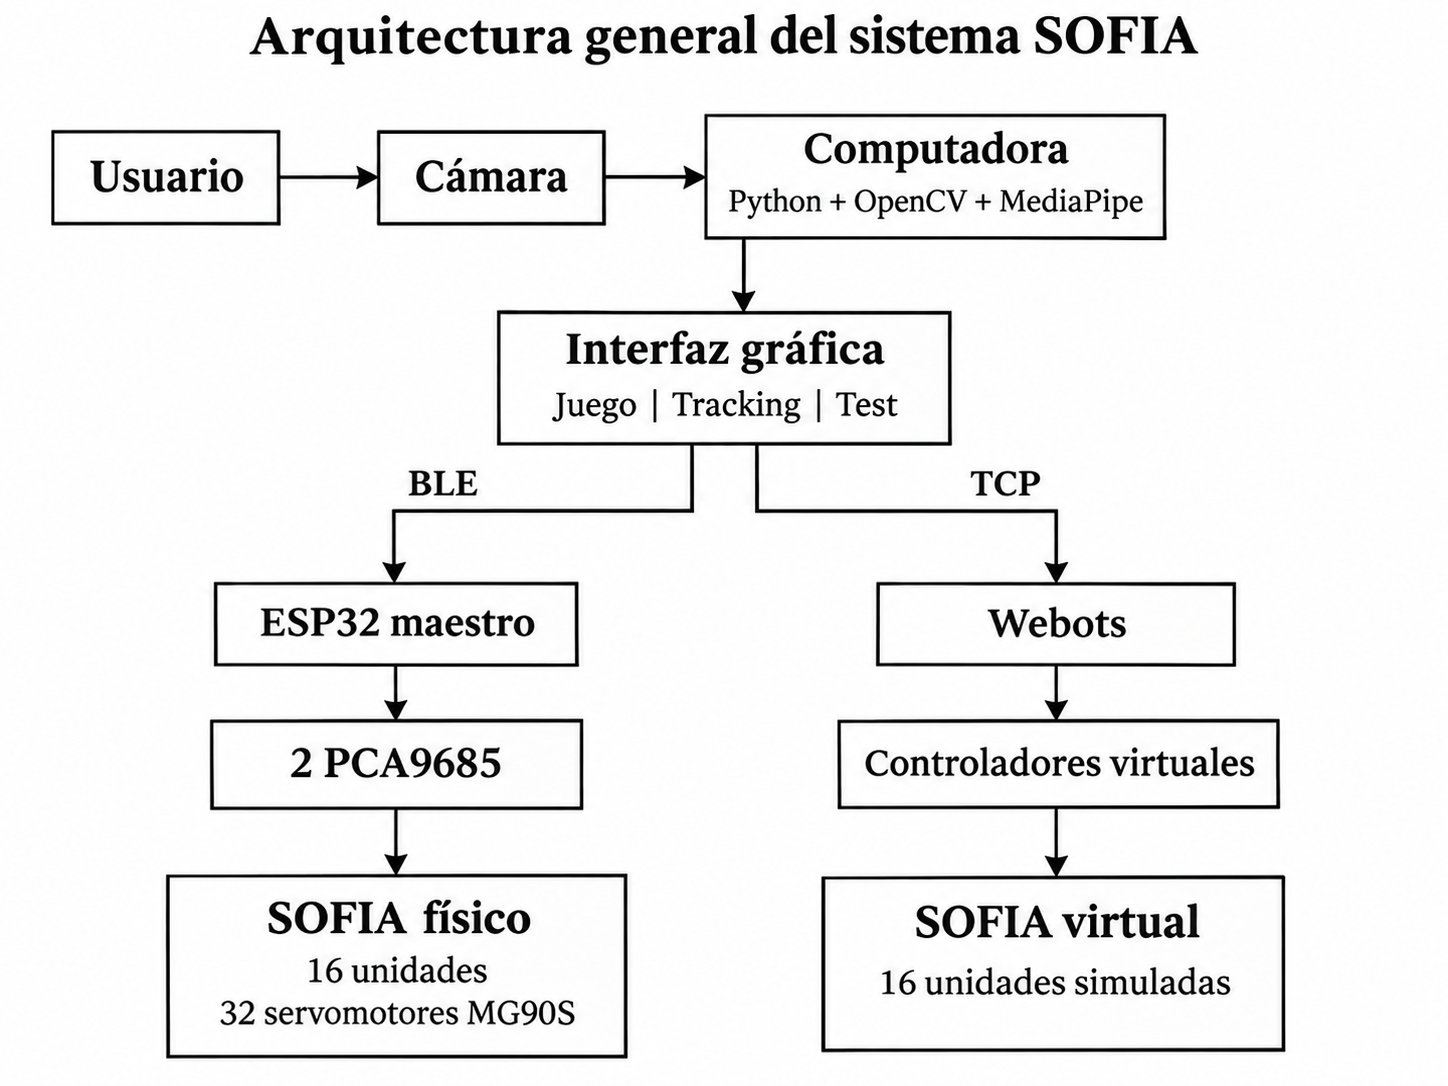
\includegraphics[width=0.95\columnwidth]{figuras/arquitectura_sofia.png}
    \caption{Arquitectura general del sistema SOFIA.}
    \label{fig:arquitectura_sofia}
\end{figure}

\section{Componentes del sistema}
\label{sec:componentes}

SOFIA está integrado por componentes mecánicos,
electrónicos y de software que permiten el funcionamiento
coordinado de la superficie cinética. Cada componente
cumple una función específica dentro del proceso de
detección, comunicación, control y ejecución de movimientos.

\subsection{Componentes mecánicos}

La estructura de SOFIA está conformada por 16 unidades
hexagonales distribuidas en un arreglo modular. Cada unidad
cuenta con dos grados de libertad rotacionales que permiten
modificar la orientación de su superficie mediante dos
servomotores.

Los principales elementos mecánicos son:

\begin{itemize}
    \item Base hexagonal de soporte.
    \item Placa superior móvil.
    \item Mecanismos de transmisión y articulaciones.
    \item Dos servomotores MG90S por unidad.
    \item Elementos de fijación y ensamble.
\end{itemize}

La coordinación de las unidades permite generar patrones
de movimiento sobre la superficie completa, así como
orientar las placas hacia un objetivo determinado.

\subsection{Componentes electrónicos}

El sistema electrónico se encarga de recibir los comandos
provenientes de la computadora y controlar los actuadores
de la superficie cinética.

Los componentes principales se presentan en la
Tabla~\ref{tab:componentes_electronicos}.

\begin{table}[!t]
    \caption{Componentes electrónicos de SOFIA}
    \label{tab:componentes_electronicos}
    \centering
    \footnotesize
    \begin{tabularx}{\columnwidth}{l c X}
        \toprule
        \textbf{Componente} & \textbf{Cant.} & \textbf{Función} \\
        \midrule
        ESP32-C3 & 1 & Control y comunicación BLE. \\
        PCA9685 & 2 & Generación de señales PWM. \\
        MG90S & 32 & Movimiento de las unidades. \\
        PCB & 1 & Interconexión electrónica. \\
        Fuente de 5 V, 2 A & 1 & Alimentación del sistema. \\
        \bottomrule
    \end{tabularx}
\end{table}

El ESP32 actúa como controlador maestro y se comunica con
los dos PCA9685 mediante el protocolo I2C. Estos dispositivos
generan las señales PWM necesarias para controlar los
32 servomotores del sistema.

\subsection{Componentes de software}

El software de SOFIA permite interpretar los movimientos
del usuario, administrar la comunicación con el controlador
electrónico y proporcionar una interfaz de operación.

Las principales herramientas utilizadas se presentan en
la Tabla~\ref{tab:componentes_software}.

\begin{table}[!t]
    \caption{Componentes de software de SOFIA}
    \label{tab:componentes_software}
    \centering
    \footnotesize
    \begin{tabularx}{\columnwidth}{l X}
        \toprule
        \textbf{Herramienta} & \textbf{Función} \\
        \midrule
        Python 3.12 & Lenguaje principal del sistema de visión. \\
        OpenCV & Captura y procesamiento de imágenes. \\
        MediaPipe & Detección corporal y de manos. \\
        NumPy & Operaciones matemáticas y geométricas. \\
        PySide6 & Desarrollo de la interfaz gráfica. \\
        Bleak & Comunicación Bluetooth Low Energy. \\
        Webots & Simulación del sistema robótico. \\
        Matplotlib & Generación de gráficas de desempeño. \\
        Openpyxl & Generación de reportes en Excel. \\
        \bottomrule
    \end{tabularx}
\end{table}

El software se encuentra organizado en módulos de detección,
interfaz, comunicación y evaluación. Esta organización
permite ejecutar los diferentes modos de operación y
registrar información sobre el desempeño del sistema.

\section{Requisitos de operación}
\label{sec:requisitos}

Antes de utilizar SOFIA, es necesario verificar que
los componentes físicos y las herramientas de software
estén disponibles y configurados correctamente.

\subsection{Requisitos de hardware}

Para operar el prototipo físico se requiere:

\begin{itemize}
    \item Una computadora con sistema operativo Windows.
    \item Una cámara web integrada o externa.
    \item Conectividad Bluetooth Low Energy (BLE).
    \item El prototipo SOFIA con sus 16 unidades instaladas.
    \item El sistema electrónico de control con ESP32-C3
    y dos módulos PCA9685.
    \item Una fuente de alimentación de 5 V y 2 A,
    correspondiente a la configuración reportada
    del prototipo.
\end{itemize}

La computadora debe contar con recursos suficientes
para ejecutar la interfaz gráfica y procesar las
imágenes de la cámara en tiempo real.

La capacidad de la fuente de alimentación debe
verificarse antes de ejecutar movimientos simultáneos
de múltiples servomotores. La especificación de 5 V
y 2 A no constituye una validación de funcionamiento
bajo la carga máxima del sistema.

\subsection{Requisitos de software}

El sistema utiliza Python 3.12 como entorno principal
de ejecución. Para utilizar la interfaz gráfica y
los módulos de visión artificial, es necesario instalar
las dependencias incluidas en el archivo
\texttt{Vision/requirements.txt}.

Las herramientas principales son:

\begin{itemize}
    \item Python 3.12.
    \item OpenCV y MediaPipe para visión artificial.
    \item PySide6 para la interfaz gráfica.
    \item Bleak para la comunicación BLE.
    \item NumPy para el procesamiento numérico.
    \item Matplotlib y Openpyxl para reportes.
\end{itemize}

Para utilizar el gemelo digital se requiere instalar
Webots y disponer de los archivos de simulación del
proyecto SOFIA.

La operación del prototipo físico no requiere
mantener Webots abierto, mientras que la simulación
puede ejecutarse sin conectar el sistema electrónico.

\subsection{Condiciones del entorno}

Para obtener un reconocimiento adecuado de los
movimientos del usuario, se recomienda utilizar
SOFIA en un espacio con iluminación uniforme
y suficiente visibilidad.

La cámara debe colocarse frente al usuario,
evitando obstáculos que oculten las manos,
los brazos o el torso durante la interacción.

También se recomienda:

\begin{itemize}
    \item Mantener una distancia que permita visualizar
    la parte superior del cuerpo.
    \item Evitar fuentes intensas de luz detrás
    del usuario.
    \item Mantener despejada el área de movimiento
    del prototipo.
    \item Colocar SOFIA sobre una superficie
    estable y nivelada.
    \item Verificar que los cables estén asegurados
    y alejados de las articulaciones móviles.
\end{itemize}

El sistema debe utilizarse en un entorno supervisado,
ya que no cuenta con un mecanismo físico dedicado
de paro de emergencia.

\subsection{Verificaciones previas}

Antes de iniciar una sesión, el usuario debe
comprobar las siguientes condiciones:

\begin{enumerate}
    \item La estructura mecánica está correctamente
    ensamblada y no presenta piezas sueltas.
    \item Los servomotores y sus conexiones no
    muestran daños visibles.
    \item La alimentación eléctrica corresponde
    a la configuración autorizada del prototipo.
    \item La cámara se encuentra conectada
    y disponible para el programa.
    \item El Bluetooth de la computadora está
    habilitado, si se utilizará el prototipo físico.
    \item El área alrededor de las unidades
    móviles está libre de obstáculos.
\end{enumerate}

Si se detectan daños, conexiones flojas,
sobrecalentamiento o movimientos anormales,
no debe iniciarse la operación hasta revisar
la condición identificada.

\section{Instalación y configuración}
\label{sec:instalacion}

Para utilizar SOFIA, es necesario disponer de los
archivos del proyecto y configurar el entorno de
ejecución de Python. El procedimiento descrito
a continuación corresponde a una computadora
con sistema operativo Windows.

\subsection{Obtención del proyecto}

Los archivos del sistema se encuentran disponibles
en el repositorio de GitHub de SOFIA.

Para obtener una copia del proyecto, abrir PowerShell
o la terminal de Visual Studio Code y ejecutar:

\begin{verbatim}
git clone https://github.com/
ale-guevarav/SOFIA.git
\end{verbatim}

El comando anterior debe ejecutarse en una sola
línea en la terminal.

Posteriormente, ingresar a la carpeta del proyecto:

\begin{verbatim}
cd SOFIA
\end{verbatim}

Si el proyecto ya se encuentra descargado, únicamente
es necesario abrir su carpeta principal desde
Visual Studio Code.

\subsection{Configuración del entorno virtual}

Se recomienda utilizar un entorno virtual para
mantener organizadas las dependencias del sistema
y evitar conflictos con otras instalaciones
de Python.

Desde la carpeta principal del repositorio,
ejecutar el siguiente comando:

\begin{verbatim}
python -m venv .venv
\end{verbatim}

En Windows, activar el entorno virtual mediante:

\begin{verbatim}
.\.venv\Scripts\Activate.ps1
\end{verbatim}

Cuando el entorno se encuentra activo, la terminal
muestra el indicador \texttt{(.venv)}.

Este procedimiento solo necesita realizarse una
vez para crear el entorno. Sin embargo, será
necesario activarlo nuevamente cuando se abra
una nueva sesión de trabajo.

\subsection{Instalación de dependencias}

Con el entorno virtual activado y desde la carpeta
principal del repositorio, instalar las bibliotecas
necesarias mediante el archivo de requisitos:

\begin{verbatim}
pip install -r Vision/requirements.txt
\end{verbatim}

Este archivo contiene las dependencias utilizadas
por el sistema de visión, la interfaz gráfica,
la comunicación BLE y la generación de reportes.

La instalación requiere acceso a Internet para
descargar los paquetes que no se encuentren
disponibles en la computadora.

Una vez finalizada, el entorno estará preparado
para ejecutar la aplicación principal.

\subsection{Ejecución de la interfaz gráfica}

Para iniciar la interfaz de SOFIA, abrir una
terminal dentro de la carpeta principal del
repositorio y verificar que el entorno virtual
se encuentre activado.

Ejecutar el siguiente comando:

\begin{verbatim}
python Vision/gui_app.py
\end{verbatim}

Si las dependencias están instaladas correctamente,
se abrirá la ventana principal del sistema.

Desde esta interfaz, el usuario podrá seleccionar
los modos de operación, activar la detección
mediante la cámara y administrar las conexiones
con el prototipo físico o la simulación.

La apertura de la interfaz no implica que el
prototipo físico ya esté conectado. La conexión
BLE debe establecerse desde la propia aplicación.

\subsection{Configuración de la cámara}

SOFIA utiliza una cámara para capturar los
movimientos del usuario durante la interacción.

Antes de iniciar la detección, se debe verificar
que la cámara esté conectada, que Windows permita
su utilización y que no se encuentre ocupada
por otra aplicación.

La configuración actual utiliza la cámara con
índice 0, correspondiente normalmente a la
primera cámara detectada por OpenCV.

Si la aplicación no consigue acceder a la
cámara, será necesario revisar su conexión,
los permisos del sistema operativo y la
configuración del dispositivo de captura.

La detección se inicia desde la interfaz gráfica
mediante el botón correspondiente.

\subsection{Preparación de Webots}

SOFIA dispone de una simulación desarrollada
en Webots que permite observar virtualmente
los movimientos de sus 16 unidades.

Para utilizar esta funcionalidad, se debe
instalar Webots y abrir el archivo de mundo
principal del proyecto:

\begin{verbatim}
Webots/Sofia/worlds/sofia.wbt
\end{verbatim}

Es necesario conservar la organización de las
carpetas del proyecto para que Webots pueda
localizar los modelos, las geometrías y los
controladores asociados con la simulación.

Una vez abierto el mundo, iniciar su ejecución
mediante el botón de reproducción de Webots.

Posteriormente, abrir la interfaz gráfica de
SOFIA y establecer la conexión con Webots
desde la sección de conexiones.

La comunicación se realiza mediante TCP local,
utilizando el puerto 5555 para el intercambio
de comandos. La visualización de la cámara
virtual utiliza una conexión independiente
por el puerto 5556.

La simulación puede utilizarse sin conectar
el prototipo físico.

\subsection{Comprobación de la instalación}

Antes de comenzar una sesión de operación,
se recomienda realizar las siguientes
verificaciones:

\begin{enumerate}
    \item Confirmar que la interfaz gráfica
    se abre sin errores.

    \item Verificar que la cámara esté
    disponible para la detección.

    \item Comprobar que los botones de los
    modos Juego, Test y Tracking aparezcan
    en la interfaz.

    \item Si se utilizará el prototipo físico,
    comprobar que la computadora tenga
    habilitado Bluetooth.

    \item Si se utilizará Webots, verificar
    que el mundo de simulación se ejecute
    correctamente.
\end{enumerate}

Si alguna de estas verificaciones falla,
se debe revisar la configuración antes
de continuar con la operación del sistema.

\section{Preparación y encendido del sistema}
\label{sec:encendido}

Antes de encender SOFIA, es necesario preparar el
área de trabajo y comprobar que los componentes
del prototipo se encuentran en condiciones
adecuadas para su utilización.

\subsection{Inspección previa del prototipo}

Colocar SOFIA sobre una superficie firme, estable
y nivelada, asegurándose de que exista espacio
suficiente para el movimiento de sus 16 unidades.

Antes de conectar la alimentación, verificar:

\begin{enumerate}
    \item Que las unidades hexagonales estén
    correctamente instaladas.
    \item Que no existan piezas sueltas o
    elementos que obstruyan el movimiento.
    \item Que las conexiones de los servomotores
    y controladores estén aseguradas.
    \item Que los cables no interfieran con
    las articulaciones.
    \item Que la fuente de alimentación
    corresponda a la configuración del prototipo.
\end{enumerate}

Si se identifica alguna anomalía, no se debe
energizar el sistema hasta realizar la revisión
correspondiente.

\subsection{Conexión de la alimentación}

El prototipo utiliza una fuente de alimentación
externa de 5 V y 2 A, conectada al sistema
electrónico de control.

El procedimiento de encendido consiste en:

\begin{enumerate}
    \item Verificar que la fuente esté
    desconectada de la alimentación eléctrica.
    \item Comprobar visualmente que las
    conexiones del prototipo estén aseguradas.
    \item Mantener las manos y otros objetos
    alejados de las unidades móviles.
    \item Conectar la fuente de alimentación
    para energizar el sistema.
    \item Observar el comportamiento inicial
    del prototipo y comprobar que no presente
    movimientos anormales.
\end{enumerate}

La conexión de la fuente constituye el
procedimiento de encendido del prototipo físico.

La capacidad de alimentación para el
funcionamiento simultáneo de todos los
servomotores requiere validación eléctrica.
Por este motivo, no deben ejecutarse pruebas
de carga máxima sin verificar previamente
la capacidad y las condiciones del sistema.

\subsection{Inicio de la aplicación}

Una vez preparado el prototipo, abrir
Visual Studio Code y acceder a la carpeta
principal del proyecto SOFIA.

Activar el entorno virtual de Python y
ejecutar el siguiente comando:

\begin{verbatim}
python Vision/gui_app.py
\end{verbatim}

La aplicación mostrará la interfaz principal,
desde la cual será posible iniciar la detección,
seleccionar los modos de operación y administrar
las conexiones del sistema.

Se recomienda comprobar que la interfaz
responda correctamente antes de enviar
comandos al prototipo físico.

\subsection{Conexión Bluetooth con el ESP32}

La comunicación entre la computadora y el
prototipo físico se realiza mediante Bluetooth
Low Energy (BLE).

Para establecer la conexión:

\begin{enumerate}
    \item Verificar que SOFIA esté encendido.
    \item Activar Bluetooth en la computadora.
    \item Abrir la interfaz gráfica de SOFIA.
    \item Localizar la sección de conexiones.
    \item Seleccionar el destino correspondiente
    al ESP32.
    \item Presionar el botón \textbf{Conectar}.
    \item Esperar a que la interfaz indique
    el estado de conexión.
\end{enumerate}

Durante la conexión, el software busca
el dispositivo BLE identificado como
\texttt{SOFIA-ESP32}.

El sistema utiliza mensajes de verificación
para comprobar la comunicación con el
controlador. La conexión debe considerarse
establecida únicamente cuando la interfaz
confirme el estado correspondiente.

Si la conexión falla, se recomienda verificar
que el prototipo esté encendido, que Bluetooth
se encuentre habilitado y que el dispositivo
esté dentro del alcance de comunicación.

\subsection{Verificación de comunicación}

Después de establecer la conexión BLE,
se recomienda comprobar que el controlador
responda correctamente.

La interfaz dispone de una función
\textbf{PING}, utilizada para verificar
la comunicación con el destino conectado.

Al realizar esta comprobación, el software
envía una solicitud al controlador y espera
una respuesta.

Una respuesta satisfactoria confirma que
existe comunicación con el dispositivo,
pero no garantiza que todos los servomotores
estén funcionando correctamente.

Antes de iniciar una sesión de movimiento,
se debe verificar visualmente que el
prototipo se encuentre en condiciones
adecuadas para operar.

\subsection{Preparación para iniciar la detección}

Una vez establecida la conexión, el usuario
puede preparar el sistema de visión artificial.

Para ello, debe colocarse frente a la cámara
y asegurarse de que las manos y el torso
sean visibles dentro de la imagen.

Posteriormente, seleccionar el modo de
operación deseado y utilizar el botón
\textbf{Iniciar} para comenzar la detección.

La interfaz permite habilitar o deshabilitar
el envío de resultados a los destinos
conectados mediante la opción
\textbf{Enviar resultados}.

Antes de utilizar el prototipo físico,
se debe comprobar que esta opción tenga
el estado adecuado para la actividad
que se desea realizar.

Durante la operación, el usuario debe
mantener las manos alejadas de las
articulaciones y superficies móviles
del prototipo.

\subsection{Consideraciones durante el encendido}

SOFIA no dispone de un botón físico
dedicado de paro de emergencia.

Por lo tanto, el usuario debe mantener
accesible el medio de desconexión
de la alimentación eléctrica y supervisar
el comportamiento del prototipo durante
toda la sesión.

El botón \textbf{Pausar} de la interfaz
detiene temporalmente el procesamiento
de detección, pero no debe considerarse
un mecanismo de paro de emergencia.

Ante ruidos inusuales, sobrecalentamiento,
movimientos inesperados o cualquier
condición que represente un riesgo,
se debe interrumpir la operación y
desconectar la alimentación, siempre
que pueda hacerse de manera segura.

No se deben manipular las conexiones
internas ni las articulaciones mientras
el sistema se encuentre energizado.

\section{Interfaz gráfica de usuario}
\label{sec:interfaz}

La interfaz gráfica de SOFIA permite controlar
las principales funciones del sistema desde una
sola ventana. Fue desarrollada en Python mediante
PySide6 y proporciona herramientas para visualizar
la cámara, seleccionar modos de operación,
administrar conexiones y consultar resultados.

La ventana principal se divide en dos áreas:
una zona de visualización ubicada a la izquierda
y un panel de controles situado a la derecha.

El panel lateral contiene las secciones de
control de detección, selección de modo,
resultados, pruebas, conexión con el robot
y bitácora de eventos.

\subsection{Visualización de la cámara}

El área principal de la interfaz muestra las
imágenes capturadas por la cámara conectada
a la computadora.

Durante la detección, el usuario puede observar
la imagen procesada por el sistema de visión,
lo que permite comprobar que sus movimientos
se encuentran dentro del campo de captura.

Cuando se activa la opción
\textbf{Ver cámara de Webots}, aparece una
segunda área de visualización para observar
la simulación.

Esta función requiere que el entorno de
Webots y su controlador de cámara estén
ejecutándose correctamente.

\subsection{Controles de detección}

La sección \textbf{Control de detección}
permite administrar el funcionamiento del
sistema de visión artificial.

Los botones disponibles son:

\begin{itemize}
    \item \textbf{Iniciar:} activa la cámara
    y comienza el procesamiento de imágenes.

    \item \textbf{Pausar:} suspende temporalmente
    el procesamiento de detección.

    \item \textbf{Reanudar:} continúa la
    detección después de una pausa.

    \item \textbf{Detener:} finaliza la sesión
    de detección y, cuando está habilitado
    el envío de resultados, solicita detener
    el movimiento de los destinos conectados.
\end{itemize}

Debajo de los botones se presenta el estado
actual del proceso de detección.

Es importante considerar que los controles
de la interfaz no sustituyen un sistema
físico de paro de emergencia.

\subsection{Selección del modo de operación}

La sección \textbf{Modo} permite seleccionar
una de las tres modalidades de funcionamiento
de SOFIA:

\begin{itemize}
    \item \textbf{Juego:} reconoce gestos
    corporales y genera los comandos
    asociados a cada postura.

    \item \textbf{Tracking:} identifica la
    posición de la mano para controlar
    la orientación de la superficie.

    \item \textbf{Test:} permite realizar
    pruebas de reconocimiento y registrar
    resultados de evaluación.
\end{itemize}

El modo Juego se encuentra seleccionado
de manera predeterminada al abrir la
aplicación.

El usuario puede cambiar de modalidad
desde esta sección. Los procedimientos
específicos de cada modo se describen
más adelante en este manual.

\subsection{Panel de resultados}

La sección \textbf{Resultado} muestra
la información obtenida durante el
procesamiento de las imágenes.

En los modos Juego y Test se presenta
el nombre de la postura identificada.

En el modo Tracking se muestran las
coordenadas normalizadas de la mano
detectada, junto con información
relacionada con su posición y orientación.

El panel también presenta indicadores
de desempeño, como:

\begin{itemize}
    \item FPS: cantidad de cuadros
    procesados por segundo.
    \item Latencia: tiempo de procesamiento
    reportado por el sistema de visión.
\end{itemize}

Estos indicadores permiten supervisar
el funcionamiento del procesamiento
visual y no representan directamente
el tiempo de movimiento de los
servomotores.

\subsection{Panel de pruebas}

La sección \textbf{Pruebas} aparece
cuando se selecciona el modo Test.

Este panel permite elegir el gesto que
se desea evaluar y comenzar una prueba
de reconocimiento.

Los gestos disponibles son:

\begin{itemize}
    \item INICIO.
    \item RECARGAR.
    \item ESCUDO.
    \item ATAQUE.
    \item FIN.
\end{itemize}

La interfaz muestra las instrucciones
de la prueba, su estado y los resultados
acumulados.

También dispone de un botón
\textbf{Cancelar} para interrumpir
una prueba en curso.

El procedimiento de evaluación
se explicará en la sección dedicada
a los modos de operación.

\subsection{Panel de conexiones}

La sección \textbf{Robot (ESP32 / Webots)}
permite administrar las conexiones
entre la interfaz gráfica y los
destinos disponibles.

Cada destino dispone de un indicador
de estado y un botón para establecer
o finalizar su conexión.

Las opciones principales son:

\begin{itemize}
    \item \textbf{ESP32:} establece la
    comunicación BLE con el prototipo físico.

    \item \textbf{Webots:} establece la
    comunicación TCP con la simulación.

    \item \textbf{PING:} verifica la
    comunicación con los destinos conectados.

    \item \textbf{Enviar resultados:}
    habilita o deshabilita el envío
    de los resultados de detección
    a los destinos conectados.

    \item \textbf{Simular canal BLE en Webots:}
    permite incorporar condiciones
    simuladas de comunicación durante
    las pruebas virtuales.

    \item \textbf{Ver cámara de Webots:}
    habilita la visualización de
    la cámara virtual.
\end{itemize}

El usuario puede conectarse únicamente
al prototipo físico, utilizar solamente
la simulación o mantener ambos destinos
conectados al mismo tiempo.

La opción \textbf{Enviar resultados}
se encuentra habilitada de manera
predeterminada.

\subsection{Bitácora de eventos}

La sección \textbf{Bitácora} permite
consultar los mensajes generados durante
el funcionamiento de la aplicación.

En ella se registran eventos relacionados
con la detección, los cambios de modo,
las conexiones y el intercambio de
comandos con los controladores.

La interfaz dispone de un campo llamado
\textbf{Condición de prueba}, donde el
usuario puede registrar información
sobre el entorno de evaluación, como
el tipo de iluminación o la presencia
de varias personas.

También incluye el botón
\textbf{Guardar resumen}, utilizado
para almacenar un resumen de los
resultados de la sesión.

Los archivos generados y sus
características se describirán
posteriormente en la sección de
registro de métricas y reportes.

\subsection{Recomendaciones de uso}

Antes de comenzar una sesión, se recomienda
verificar el estado de las conexiones y
seleccionar el modo de operación adecuado.

Si se desea evaluar únicamente el
reconocimiento de gestos sin provocar
movimientos físicos, se debe deshabilitar
\textbf{Enviar resultados} y comprobar
que no existan movimientos pendientes.

Para finalizar una sesión, se recomienda
mantener habilitado el envío de comandos,
utilizar \textbf{Detener}, comprobar
visualmente que el prototipo haya cesado
su movimiento y desconectar los destinos
antes de cerrar la aplicación.

El botón \textbf{Detener} no constituye
una función de seguridad independiente.
Además, su solicitud de detención
depende de que exista una detección
activa y de que esté habilitada
la opción \textbf{Enviar resultados}.

La desconexión de la alimentación
debe realizarse siguiendo las
consideraciones de seguridad
establecidas para el prototipo.

\section{Modos de operación}
\label{sec:modos_operacion}

SOFIA dispone de tres modos de operación que permiten
interactuar con la superficie cinética y evaluar el
funcionamiento del sistema de visión artificial.

Los modos disponibles son Juego, Tracking y Test.
Cada uno utiliza la cámara para interpretar los
movimientos del usuario, pero presenta diferencias
en el procesamiento y en los resultados generados.

La selección del modo se realiza desde el panel
correspondiente de la interfaz gráfica.

\subsection{Modo Juego}

El modo Juego permite controlar SOFIA mediante el
reconocimiento de cinco gestos corporales:
INICIO, RECARGAR, ESCUDO, ATAQUE y FIN.

El sistema procesa las imágenes capturadas por la
cámara mediante MediaPipe y determina si el usuario
está realizando alguno de los gestos definidos.

Cuando se identifica un gesto válido y diferente
del último reconocido, la aplicación genera el
comando correspondiente y lo envía a los destinos
conectados, siempre que esté habilitada la opción
\textbf{Enviar resultados}.

\subsubsection{Procedimiento de operación}

\begin{enumerate}
    \item Abrir la interfaz gráfica de SOFIA.
    \item Seleccionar el modo \textbf{Juego}.
    \item Establecer la conexión con ESP32,
    Webots o ambos, según corresponda.
    \item Verificar la opción
    \textbf{Enviar resultados}.
    \item Colocarse frente a la cámara.
    \item Presionar el botón \textbf{Iniciar}.
    \item Realizar uno de los gestos definidos.
    \item Observar el resultado del reconocimiento
    y la respuesta del destino conectado.
\end{enumerate}

El panel de resultados muestra el nombre del
gesto identificado y el estado de detección
de la persona.

La respuesta mecánica depende del patrón
asignado al gesto reconocido.

\subsection{Modo Tracking}

El modo Tracking permite controlar la orientación
de las unidades de SOFIA mediante el seguimiento
de la posición de la mano del usuario.

Durante este modo, el sistema de visión identifica
la posición de la mano y obtiene coordenadas
normalizadas que representan su desplazamiento
respecto al centro de la imagen.

Estas coordenadas se utilizan para generar comandos
de seguimiento que son transmitidos al controlador
físico o al entorno de simulación.

En Webots, el seguimiento se representa mediante
una esfera virtual cuya posición depende del
movimiento de la mano. Las unidades de la
superficie orientan sus placas hacia dicha esfera.

\subsubsection{Procedimiento de operación}

\begin{enumerate}
    \item Abrir la interfaz gráfica.
    \item Seleccionar el modo \textbf{Tracking}.
    \item Establecer la conexión con el destino
    que se desea utilizar.
    \item Activar \textbf{Enviar resultados}
    si se desea controlar el destino conectado.
    \item Presionar \textbf{Iniciar}.
    \item Colocar una mano frente a la cámara.
    \item Desplazar la mano horizontal y
    verticalmente dentro del campo de visión.
    \item Observar el seguimiento de la
    superficie física o virtual.
\end{enumerate}

\subsubsection{Información mostrada}

Durante el seguimiento, la interfaz presenta
las coordenadas de la mano, su posición
normalizada, la magnitud del desplazamiento
y el ángulo calculado respecto al centro
de referencia.

Las coordenadas normalizadas utilizan un
intervalo aproximado de -1 a 1 para representar
la posición horizontal y vertical.

Cuando no existe una posición de mano disponible,
la interfaz muestra el mensaje
\textbf{Sin mano}.

\subsection{Modo Test}

El modo Test permite realizar pruebas controladas
del sistema de reconocimiento de gestos.

Su objetivo es comprobar si el software identifica
correctamente una postura solicitada y registrar
información sobre el desempeño de la detección.

La interfaz permite evaluar individualmente los
cinco gestos disponibles en el modo Juego.

\subsubsection{Procedimiento de operación}

\begin{enumerate}
    \item Abrir la interfaz gráfica de SOFIA.
    \item Seleccionar el modo \textbf{Test}.
    \item Presionar el botón \textbf{Iniciar}
    para activar la detección.
    \item Seleccionar el gesto que se desea evaluar.
    \item Esperar la cuenta regresiva de
    tres segundos.
    \item Cuando aparezca la indicación
    \textbf{YA}, realizar el gesto solicitado.
    \item Observar el resultado de la prueba.
    \item Repetir el procedimiento para realizar
    nuevas evaluaciones.
\end{enumerate}

Cada prueba dispone de un periodo de seis segundos
para identificar el gesto solicitado.

Si el sistema reconoce el gesto esperado,
la interfaz muestra \textbf{ACIERTO}.
En caso contrario, muestra \textbf{FALLO}.

El panel también presenta los intentos realizados,
la cantidad de aciertos y otros indicadores
obtenidos durante la evaluación.

\subsubsection{Cancelación de una prueba}

Para interrumpir una evaluación en curso,
el usuario puede presionar el botón
\textbf{Cancelar} del panel de pruebas.

Esta acción cancela la evaluación seleccionada,
pero no constituye un procedimiento de
desconexión del prototipo físico.

\subsection{Cambio entre modos}

La interfaz permite cambiar de modalidad
mediante las opciones Juego, Tracking y Test.

Al seleccionar un modo diferente, la aplicación
actualiza el procesamiento de visión y envía
el comando de cambio de modalidad a los
destinos conectados, siempre que el envío
de resultados se encuentre habilitado.

Antes de cambiar de modo durante una operación
física, se recomienda comprobar que la superficie
no esté ejecutando un movimiento que pueda
representar un riesgo.

En particular, durante las pruebas de reconocimiento
que no requieran actuación mecánica, se recomienda
deshabilitar \textbf{Enviar resultados} antes
de iniciar la evaluación.

La selección de un modo no sustituye el
procedimiento de detención ni la desconexión
de alimentación del prototipo.

\subsection{Operación física y virtual}

Los tres modos pueden utilizarse con los
destinos de comunicación disponibles.

Cuando se establece una conexión con el ESP32,
los comandos se transmiten mediante BLE al
prototipo físico.

Cuando se establece una conexión con Webots,
los comandos se transmiten mediante TCP al
entorno de simulación.

La interfaz también permite mantener ambos
destinos conectados simultáneamente y enviarles
los mismos resultados de detección.

Sin embargo, la recepción de un comando no
garantiza que los movimientos físicos y
virtuales ocurran exactamente al mismo tiempo.

El usuario debe verificar visualmente el
comportamiento de cada destino durante
la operación.

\section{Gestos y patrones de movimiento}
\label{sec:gestos_patrones}

SOFIA permite interactuar con la superficie
cinética mediante cinco gestos: INICIO,
RECARGAR, ESCUDO, ATAQUE y FIN.

Cada gesto reconocido se asocia con un comando
de movimiento que determina la respuesta de
las unidades mecánicas del sistema.

El reconocimiento depende de la posición
corporal del usuario, mientras que la ejecución
del patrón depende del controlador y del
destino seleccionado.

Para utilizar esta funcionalidad, es necesario
activar el modo Juego, iniciar la detección
y habilitar el envío de resultados cuando
se desee controlar el prototipo físico
o la simulación.

\subsection{Patrones disponibles}

Los cinco comandos de SOFIA generan
trayectorias de movimiento diferentes,
las cuales se resumen en la
Tabla~\ref{tab:patrones_sofia}.

\begin{table}[!t]
    \caption{Gestos y patrones de SOFIA}
    \label{tab:patrones_sofia}
    \centering
    \footnotesize
    \begin{tabularx}{\columnwidth}{l X}
        \toprule
        \textbf{Gesto} & \textbf{Patrón asociado} \\
        \midrule
        INICIO & Movimiento vertical de
        arriba hacia abajo. \\
        RECARGAR & Recorrido circular
        por las unidades del perímetro. \\
        ESCUDO & Trayectoria con
        forma de rombo. \\
        ATAQUE & Trayectoria con
        forma de letra L. \\
        FIN & Movimiento horizontal
        de izquierda a derecha. \\
        \bottomrule
    \end{tabularx}
\end{table}

\subsection{Descripción de los movimientos}

\subsubsection{INICIO}

El patrón INICIO genera un movimiento
vertical que comienza en el centro,
se dirige hacia arriba, continúa hacia
abajo y finalmente regresa al centro.

\subsubsection{RECARGAR}

El patrón RECARGAR produce un efecto
circular sobre el perímetro de la superficie.

Las unidades exteriores se inclinan
secuencialmente hacia afuera, creando
un movimiento en sentido horario que
completa dos vueltas.

\subsubsection{ESCUDO}

El patrón ESCUDO describe una trayectoria
con forma de rombo. El recorrido comienza
en la parte superior, continúa hacia
la derecha, desciende, se desplaza
hacia la izquierda y vuelve al inicio.

\subsubsection{ATAQUE}

El patrón ATAQUE genera una trayectoria
con forma de letra L. El movimiento
comienza en la zona superior izquierda,
desciende verticalmente y después
se desplaza hacia la derecha.

\subsubsection{FIN}

El patrón FIN produce movimientos
horizontales alternados, de izquierda
a derecha y nuevamente en sentido
contrario, como una despedida.

\subsection{Coordinación de las unidades}

En el modelo de patrones de SOFIA,
las trayectorias se representan mediante
una esfera virtual que se desplaza
sobre la superficie.

Para los patrones INICIO, ESCUDO,
ATAQUE y FIN, se define un conjunto
de unidades que pueden participar
en el movimiento.

Durante el recorrido, se seleccionan
hasta tres unidades cercanas a la
posición de la esfera virtual para
calcular sus orientaciones objetivo.

El patrón RECARGAR utiliza una lógica
diferente, basada en el movimiento
secuencial de las unidades exteriores.

Esta estrategia permite generar
movimientos localizados y coordinados,
en lugar de asignar necesariamente
la misma inclinación a toda la superficie.

El modelo de patrones contempla una
amplitud objetivo de hasta 20 grados,
con actualizaciones cada 20 ms.
Estos parámetros corresponden al
modelo documentado y no sustituyen
la verificación de los límites
mecánicos del prototipo físico.

\subsection{Procedimiento de ejecución}

Para ejecutar un patrón mediante
reconocimiento de gestos:

\begin{enumerate}
    \item Iniciar la interfaz gráfica.
    \item Establecer la conexión con
    ESP32, Webots o ambos.
    \item Seleccionar el modo Juego.
    \item Habilitar Enviar resultados.
    \item Iniciar la detección.
    \item Colocarse frente a la cámara.
    \item Realizar uno de los gestos
    reconocidos por el sistema.
    \item Verificar el resultado
    mostrado en la interfaz.
    \item Observar la ejecución del
    patrón correspondiente.
\end{enumerate}

Si no se reconoce el gesto, se
recomienda revisar la iluminación,
la posición del usuario y la
visibilidad de sus brazos y manos.

Durante la ejecución de los patrones,
el usuario debe mantener despejada
la zona de movimiento del prototipo.

\subsection{Consideraciones de funcionamiento}

Los patrones dependen de la modalidad
seleccionada y de la configuración
del controlador utilizado.

El reconocimiento de un gesto no
garantiza por sí mismo que el
movimiento físico se haya completado.

Para comprobar el funcionamiento,
el usuario debe verificar tanto
el resultado mostrado en la interfaz
como la respuesta observable del
prototipo o la simulación.

Si el patrón no se ejecuta,
se recomienda revisar el estado
de conexión, la opción Enviar
resultados y los mensajes
de la bitácora.

\section{Simulación y gemelo digital}
\label{sec:simulacion}

SOFIA cuenta con un entorno de simulación
desarrollado en Webots que permite reproducir
virtualmente el comportamiento de sus
16 unidades mecánicas.

Cada unidad dispone de dos grados de libertad
y puede modificar la orientación de su placa
superior mediante motores virtuales.

La simulación permite observar los patrones
de movimiento, realizar pruebas de seguimiento
y comprobar la comunicación con la interfaz
gráfica sin utilizar el prototipo físico.

También es posible mantener conectados
simultáneamente el prototipo físico y la
simulación, utilizando ambos como parte
de un entorno de gemelo digital.

\subsection{Componentes de la simulación}

El entorno virtual está integrado por los
siguientes elementos:

\begin{itemize}
    \item \textbf{Mundo virtual:} contiene
    las 16 unidades mecánicas, una esfera
    de referencia y una cámara cenital.

    \item \textbf{Controlador maestro:}
    recibe los comandos de la interfaz,
    verifica las tramas de comunicación
    y administra el comportamiento general.

    \item \textbf{Controladores de unidades:}
    calculan y ejecutan los movimientos
    de las placas virtuales.

    \item \textbf{Cámara virtual:} captura
    una vista superior de la superficie
    y la transmite a la interfaz gráfica.
\end{itemize}

El procesamiento de visión artificial
continúa ejecutándose en la computadora
mediante la cámara real y MediaPipe.
Webots recibe los resultados procesados,
pero no realiza directamente el
reconocimiento de gestos del usuario.

\subsection{Inicio de la simulación}

Para ejecutar SOFIA en Webots se debe
realizar el siguiente procedimiento:

\begin{enumerate}
    \item Abrir Webots en la computadora.

    \item Desde el programa, abrir el mundo:

    \texttt{Webots/Sofia/worlds/sofia.wbt}

    \item Verificar que se visualicen las
    16 unidades de la superficie cinética.

    \item Iniciar la simulación mediante
    el botón de reproducción.

    \item Comprobar que los controladores
    se ejecuten sin errores.

    \item Abrir la interfaz gráfica
    mediante el comando:

    \texttt{python Vision/gui\_app.py}

    \item Localizar el panel
    \textbf{Robot (ESP32 / Webots)}.

    \item Presionar \textbf{Conectar}
    en la opción correspondiente a Webots.
\end{enumerate}

Si la conexión se establece correctamente,
la interfaz mostrará el estado del
destino virtual.

Una vez conectado, el usuario podrá
seleccionar el modo de operación
e iniciar la detección.

\subsection{Comunicación con Webots}

La comunicación entre la interfaz gráfica
y Webots se realiza mediante una conexión
TCP local.

El sistema utiliza dos canales
independientes:

\begin{itemize}
    \item \textbf{Puerto 5555:}
    transmisión de comandos y respuestas
    entre la interfaz y el controlador
    maestro de la simulación.

    \item \textbf{Puerto 5556:}
    transmisión de imágenes desde
    la cámara virtual hacia la interfaz.
\end{itemize}

Los comandos utilizan el mismo formato
de protocolo definido para la comunicación
con el ESP32.

El controlador maestro puede responder
con mensajes de confirmación o error,
lo que permite supervisar el intercambio
de información desde la bitácora.

La conexión se realiza normalmente
mediante la dirección local
\texttt{127.0.0.1}.

\subsection{Visualización de la cámara virtual}

Webots incorpora una cámara cenital que
permite observar la superficie desde
una perspectiva superior.

Para mostrar esta vista en la
interfaz gráfica:

\begin{enumerate}
    \item Iniciar el mundo de simulación.
    \item Abrir la interfaz de SOFIA.
    \item Localizar el panel de conexiones.
    \item Activar la casilla
    \textbf{Ver cámara de Webots}.
    \item Verificar que aparezca
    la imagen de la superficie virtual.
\end{enumerate}

La imagen de Webots se presenta en
un área adicional de visualización,
independiente del video de la cámara real.

Si la cámara virtual no está disponible,
la conexión principal de comandos
puede continuar funcionando.

\subsection{Modos de operación en Webots}

La simulación permite utilizar los modos
Juego, Tracking y Test mediante los
comandos recibidos desde la interfaz.

\subsubsection{Modo Juego}

Al reconocer un gesto, la interfaz
envía el comando correspondiente
a Webots.

Las unidades virtuales ejecutan el
patrón asociado al gesto recibido,
de acuerdo con la implementación
del controlador de simulación.

\subsubsection{Modo Tracking}

Durante el seguimiento, la posición
de la mano controla el desplazamiento
de una esfera virtual.

Las 16 unidades de SOFIA modifican
su orientación para apuntar hacia
la posición de dicha esfera.

\subsubsection{Modo Test}

El sistema permite evaluar el
reconocimiento de gestos mientras
Webots permanece conectado.

En este modo, la esfera virtual
de seguimiento permanece oculta
y las unidades se mantienen
en su posición de referencia,
salvo que se reciban otros
comandos de movimiento.

\subsection{Funcionamiento como gemelo digital}

La interfaz de SOFIA permite conectar
simultáneamente el ESP32 y Webots.

En esta configuración, los resultados
del procesamiento de visión pueden
enviarse a ambos destinos mediante
sus respectivos enlaces de comunicación.

Para utilizar esta función:

\begin{enumerate}
    \item Encender el prototipo físico
    y verificar sus condiciones de seguridad.

    \item Iniciar el mundo de Webots.

    \item Abrir la interfaz gráfica.

    \item Establecer la conexión BLE
    con el ESP32.

    \item Establecer la conexión TCP
    con Webots.

    \item Habilitar
    \textbf{Enviar resultados}.

    \item Seleccionar el modo deseado
    e iniciar la detección.

    \item Observar la respuesta de ambos
    sistemas durante la interacción.
\end{enumerate}

La bitácora identifica los mensajes
procedentes de ESP32 y Webots,
permitiendo consultar las respuestas
de cada destino.

Aunque ambos reciben los mismos
comandos, sus movimientos no
necesariamente ocurren de manera
sincronizada debido a diferencias
de comunicación, procesamiento
y actuación.

\subsection{Simulación del canal de comunicación}

La interfaz dispone de una opción
denominada \textbf{Simular canal BLE en Webots}.

Esta función permite introducir
condiciones artificiales de comunicación
en el enlace virtual, como retrasos,
pérdidas de mensajes y alteraciones
en las tramas transmitidas.

La configuración documentada contempla
aproximadamente 30 ms de retraso,
una probabilidad de pérdida del 3\%
y una probabilidad de corrupción del 2\%.

Estas condiciones permiten observar
el comportamiento del protocolo
ante errores de transmisión, así
como las respuestas y reintentos
registrados en la bitácora.

Esta función se utiliza únicamente
para evaluación del enlace virtual
y no modifica las condiciones reales
de la comunicación BLE del ESP32.

\subsection{Consideraciones de uso}

Antes de utilizar Webots, se debe
verificar que los archivos del modelo
y los controladores estén disponibles
en la estructura del proyecto.

Si se modifican los controladores
desarrollados en C++, puede ser
necesario compilarlos nuevamente
desde el editor de Webots mediante
la opción \textbf{Clean \& Build}.

Si la simulación no responde,
se recomienda comprobar que el mundo
esté ejecutándose, que los puertos
de comunicación estén disponibles
y que la interfaz indique una
conexión activa.

Los resultados obtenidos en Webots
representan el comportamiento del
modelo virtual y no sustituyen
las pruebas de funcionamiento
del prototipo físico.

\section{Diagnóstico de orientación mediante CNN}
\label{sec:diagnostico_cnn}

SOFIA contempla un sistema experimental de
diagnóstico de orientación basado en redes
neuronales convolucionales (CNN).

Esta funcionalidad está orientada al análisis
de la posición de las unidades de la superficie
mediante información visual, con el propósito
de estudiar posibles diferencias entre las
orientaciones esperadas y las observadas.

El desarrollo y las pruebas de esta
funcionalidad se han realizado en un
entorno de simulación, por lo que sus
resultados no deben interpretarse como
una validación del sistema físico.

\subsection{Entorno de simulación}

El proyecto dispone de escenarios de Webots
destinados a la generación de información
visual y al estudio de la orientación
de las unidades mecánicas.

Estos escenarios permiten representar
diferentes configuraciones de la superficie
sin requerir movimientos del prototipo físico.

Los archivos de simulación relacionados
con esta funcionalidad incluyen:

\begin{itemize}
    \item \texttt{sofia\_dataset.wbt}
    \item \texttt{sofia\_diagnostico\_vivo.wbt}
\end{itemize}

Estos archivos se encuentran dentro
del directorio de mundos de Webots
del proyecto SOFIA.

\subsection{Alcance del diagnóstico}

El diagnóstico visual mediante CNN
constituye una funcionalidad experimental
separada de los procedimientos habituales
de operación de SOFIA.

Su propósito es apoyar el análisis
de las orientaciones de las unidades
dentro del entorno virtual.

Actualmente, este manual no considera
el diagnóstico mediante CNN como
un requisito para utilizar los modos
Juego, Tracking o Test.

Tampoco se considera una función
de seguridad ni un mecanismo autónomo
de corrección de los servomotores
del prototipo físico.

La aplicación de esta funcionalidad
sobre el sistema real requiere
validaciones adicionales.

\subsection{Consideraciones para el usuario}

Para la operación convencional de SOFIA
no es necesario ejecutar el módulo
experimental de diagnóstico mediante CNN.

Las actividades relacionadas con esta
funcionalidad deben realizarse en el
entorno de simulación correspondiente
y siguiendo la configuración específica
del módulo de diagnóstico.

Los resultados obtenidos deben
interpretarse como información
experimental del modelo virtual.

No se deben aplicar correcciones
mecánicas o electrónicas al prototipo
físico basándose únicamente en estos
resultados.

\section{Registro de métricas y reportes}
\label{sec:metricas_reportes}

SOFIA incorpora herramientas para registrar
información durante las sesiones de detección
y las pruebas de funcionamiento.

El sistema permite almacenar las posturas
reconocidas, los comandos transmitidos,
los eventos de comunicación y diferentes
indicadores de desempeño.

Esta información facilita la revisión
de los resultados obtenidos y la
identificación de posibles problemas
durante la operación.

\subsection{Métricas de desempeño}

Durante una sesión, SOFIA puede registrar
indicadores relacionados con el procesamiento
de imágenes y el reconocimiento de gestos.

Las principales métricas son:

\begin{itemize}
    \item \textbf{FPS:} cantidad de cuadros
    procesados por segundo.

    \item \textbf{Latencia de procesamiento:}
    tiempo requerido para procesar
    las imágenes capturadas.

    \item \textbf{Tiempo de respuesta:}
    tiempo registrado durante las
    pruebas de reconocimiento.

    \item \textbf{Tasa de acierto:}
    proporción de pruebas en las
    que se reconoce el gesto esperado.

    \item \textbf{Precisión, recall y F1:}
    indicadores utilizados para evaluar
    el reconocimiento de las posturas.

    \item \textbf{Matriz de confusión:}
    comparación entre los gestos esperados
    y los resultados identificados.
\end{itemize}

La disponibilidad de estas métricas
depende de los datos registrados
durante cada sesión.

\subsection{Registro de sesiones}

La interfaz gráfica incorpora un
registro de eventos que permite
conservar información sobre el
funcionamiento del sistema.

Los archivos se almacenan dentro
del directorio:

\begin{verbatim}
Vision/metrics/sesiones/
\end{verbatim}

Cada sesión utiliza una carpeta
identificada mediante su fecha y hora.

Dentro de esta carpeta pueden
generarse los siguientes archivos:

\begin{itemize}
    \item \texttt{posturas.csv}:
    cambios de postura detectados.

    \item \texttt{comandos.csv}:
    comandos enviados, respuestas
    y tiempos de comunicación.

    \item \texttt{eventos.csv}:
    conexiones, desconexiones
    y eventos de funcionamiento.

    \item \texttt{bitacora.txt}:
    mensajes registrados por
    la interfaz gráfica.

    \item \texttt{resumen.md}:
    resumen de la sesión en Markdown.

    \item \texttt{resumen.json}:
    información estructurada
    del resumen de sesión.
\end{itemize}

La carpeta se crea cuando se registra
el primer evento. Los archivos
disponibles pueden variar según
las actividades realizadas.

\subsection{Condiciones de prueba}

La interfaz dispone de un campo
denominado \textbf{Condición de prueba},
que permite identificar las
circunstancias de una evaluación.

El usuario puede introducir
descripciones como iluminación baja,
presencia de varias personas
o movimientos rápidos.

Esta información se utiliza para
clasificar los registros y comparar
resultados obtenidos bajo diferentes
condiciones.

Para registrar una condición,
se debe escribir su descripción
en el campo correspondiente
y confirmar el cambio antes
de comenzar la prueba.

\subsection{Guardado del resumen}

Para guardar un resumen de los
eventos registrados, el usuario
debe seguir este procedimiento:

\begin{enumerate}
    \item Abrir la interfaz gráfica.
    \item Realizar la sesión de
    detección o evaluación.
    \item Localizar la sección
    de bitácora.
    \item Presionar el botón
    \textbf{Guardar resumen}.
    \item Revisar los archivos
    generados en la carpeta
    correspondiente a la sesión.
\end{enumerate}

Esta función permite almacenar
los registros agrupados por
condición de prueba, incluyendo
información sobre posturas,
comandos, eventos y comunicación.

El resumen también puede
guardarse al cerrar la aplicación.

\subsection{Generación de reportes}

SOFIA dispone de un módulo que
permite generar reportes a partir
de las métricas recopiladas.

Cuando una sesión contiene datos
de evaluación, el sistema puede
generar un archivo JSON con
la información registrada.

Los archivos de métricas se
almacenan en el directorio:

\begin{verbatim}
Vision/metrics/
\end{verbatim}

Los reportes correspondientes
se organizan dentro de:

\begin{verbatim}
Vision/metrics/reportes/
\end{verbatim}

Cada reporte puede incluir:

\begin{itemize}
    \item \texttt{reporte.xlsx}:
    archivo de Excel con tablas
    e indicadores de desempeño.

    \item \texttt{reporte.md}:
    resumen de los resultados
    en formato Markdown.

    \item Carpeta \texttt{graficas}:
    representaciones visuales
    de los resultados.
\end{itemize}

Los reportes permiten consultar
el comportamiento del sistema
durante las pruebas realizadas,
sin necesidad de procesar
manualmente todos los registros.

\subsection{Generación manual de reportes}

Si se dispone de un archivo JSON
de métricas, es posible generar
nuevamente su reporte.

Para ello, abrir una terminal
desde la carpeta \texttt{Vision}
del repositorio y ejecutar:

\begin{verbatim}
python -m evaluacion.generate_report
\end{verbatim}

Cuando no se especifica un archivo,
el programa utiliza la sesión
de métricas más reciente disponible.

El usuario también puede indicar
la ruta de un archivo JSON
para procesar una sesión específica.

Los resultados se guardan en
la carpeta de reportes,
organizados por sesión.

\subsection{Interpretación de los registros}

Los registros de comunicación
permiten consultar información
sobre los comandos enviados
y las respuestas de los
destinos conectados.

Entre los tiempos disponibles
se encuentran:

\begin{itemize}
    \item \texttt{rtt\_ms}:
    tiempo entre el envío
    y la respuesta del comando
    en el intento registrado.

    \item \texttt{cola\_ms}:
    tiempo desde la solicitud
    del comando hasta su
    confirmación, incluyendo
    posibles esperas y reintentos.

    \item \texttt{ciclo\_ms}:
    suma del procesamiento visual
    y el tiempo de comunicación
    asociado al comando.
\end{itemize}

Estos valores permiten evaluar
el desempeño del procesamiento
y la comunicación.

Sin embargo, una confirmación
de recepción no garantiza
que el movimiento físico
se haya completado.

Por ello, los registros deben
interpretarse junto con la
observación del comportamiento
del prototipo.

\section{Apagado del sistema}
\label{sec:apagado}

El apagado de SOFIA debe realizarse
de manera ordenada para finalizar
la detección, cerrar las conexiones
activas y retirar la alimentación
del prototipo físico.

El procedimiento recomendado es:

\begin{enumerate}
    \item Finalizar la interacción
    y mantener despejada el área
    de movimiento del prototipo.

    \item Verificar que la opción
    \textbf{Enviar resultados}
    esté habilitada.

    \item Presionar \textbf{Detener}
    para finalizar la detección
    y solicitar la detención
    de los destinos conectados.

    \item Comprobar visualmente que
    las unidades hayan dejado
    de moverse.

    \item Guardar el resumen
    de la sesión, si corresponde.

    \item Desconectar los destinos
    ESP32 y Webots desde la interfaz.

    \item Cerrar la aplicación
    de SOFIA.

    \item Desconectar la fuente
    de alimentación del prototipo
    físico de manera segura.
\end{enumerate}

Este procedimiento corresponde
al apagado normal del sistema
y no sustituye una acción
de emergencia.

\subsection{Detención de la detección}

El botón \textbf{Detener} permite
finalizar el procesamiento de imágenes
y cerrar la sesión de detección.

Cuando existen destinos conectados
y la opción \textbf{Enviar resultados}
está habilitada, la aplicación
también transmite una solicitud
de detención.

Si esta opción está deshabilitada,
no debe suponerse que el botón
enviará un comando de detención
al prototipo.

Por otra parte, el botón
\textbf{Pausar} únicamente suspende
temporalmente la detección y
no constituye un mecanismo
de detención física.

La respuesta del controlador
debe comprobarse visualmente
antes de continuar con el apagado.

\subsection{Desconexión de dispositivos}

Una vez finalizada la detección
y comprobado que las unidades
han dejado de moverse, el usuario
puede cerrar las conexiones activas.

Para desconectar el prototipo físico:

\begin{enumerate}
    \item Localizar el panel
    \textbf{Robot (ESP32 / Webots)}.

    \item Identificar la conexión
    correspondiente al ESP32.

    \item Presionar
    \textbf{Desconectar}.

    \item Verificar el cambio
    de estado de la conexión.
\end{enumerate}

Si Webots se encuentra conectado,
realizar el mismo procedimiento
con el destino virtual.

La desconexión de BLE o TCP
no equivale a retirar la
alimentación eléctrica
del prototipo.

\subsection{Cierre de la aplicación}

Después de finalizar la detección
y desconectar los destinos,
se puede cerrar la ventana
principal de SOFIA.

Durante el cierre, la aplicación
finaliza sus procesos de
detección y comunicación
y guarda el resumen de
la sesión cuando corresponde.

No se debe utilizar el cierre
de la ventana como sustituto
del procedimiento de detención.

Si Webots se encuentra abierto,
se recomienda detener la simulación
y cerrar el programa una vez
finalizadas las pruebas.

\subsection{Desconexión de la alimentación}

El prototipo físico se enciende
y apaga mediante la conexión
y desconexión de su fuente
de alimentación externa.

Para completar el apagado normal,
comprobar primero que la superficie
haya detenido su movimiento.

Posteriormente, desconectar
la alimentación utilizando
el medio previsto para ello,
sin manipular las conexiones
internas del circuito energizado.

No se deben retirar servomotores,
modificar el cableado ni realizar
ajustes mecánicos mientras
el prototipo permanezca conectado
a la fuente eléctrica.

Después de desconectar la fuente,
se puede proceder a la inspección
o mantenimiento del sistema.

\subsection{Detención ante una anomalía}

Si durante la operación se presentan
movimientos inesperados, ruidos
inusuales, sobrecalentamiento
o señales de falla eléctrica,
se debe interrumpir la actividad.

Debido a que SOFIA no dispone
de un paro de emergencia físico,
los botones de la interfaz
no deben considerarse
dispositivos de seguridad.

Ante una situación de riesgo,
el usuario debe alejarse
de las partes móviles y
desconectar la alimentación
por un medio accesible,
siempre que pueda hacerlo
sin exponerse al peligro.

Una vez desenergizado el sistema,
se debe identificar la causa
de la anomalía antes de volver
a utilizar el prototipo.

\section{Consideraciones de seguridad}
\label{sec:seguridad}

SOFIA es un prototipo robótico experimental
que integra componentes electrónicos,
mecánicos y sistemas de visión artificial.

Su utilización requiere supervisión,
especialmente durante la ejecución
de movimientos físicos.

Antes de operar el sistema, el usuario
debe conocer los procedimientos de
encendido, funcionamiento y apagado
descritos en este manual.

El prototipo no dispone de un mecanismo
físico dedicado de paro de emergencia,
por lo que no debe utilizarse en
actividades que requieran funciones
de seguridad certificadas.

\subsection{Seguridad mecánica}

Las 16 unidades de SOFIA contienen
mecanismos articulados accionados
por servomotores.

Durante su funcionamiento, estas
articulaciones pueden generar puntos
de atrapamiento entre las piezas móviles.

Para reducir los riesgos mecánicos,
se recomienda:

\begin{itemize}
    \item Mantener las manos alejadas
    de las articulaciones durante
    el movimiento.

    \item Evitar colocar objetos
    sobre las unidades móviles.

    \item No intentar detener
    manualmente los servomotores.

    \item Comprobar que las piezas
    estén correctamente aseguradas.

    \item Mantener despejada
    el área de operación.
\end{itemize}

Los ajustes mecánicos deben realizarse
únicamente cuando el prototipo esté
desconectado de la alimentación eléctrica.

\subsection{Seguridad eléctrica}

SOFIA utiliza una fuente externa
de alimentación de 5 V y 2 A,
correspondiente a la configuración
reportada del prototipo.

Debido a que el sistema incorpora
32 servomotores, es necesario
verificar que la alimentación
disponible sea adecuada para
las condiciones de operación.

No se debe asumir que la fuente
reportada permite accionar todos
los servomotores simultáneamente
bajo carga máxima.

Durante la utilización del sistema
se recomienda:

\begin{itemize}
    \item Verificar la polaridad
    y el estado de las conexiones.

    \item No manipular el cableado
    mientras el sistema esté
    energizado.

    \item Evitar cortocircuitos
    y conexiones flojas.

    \item Suspender las pruebas
    ante sobrecalentamiento,
    olores anormales o fallas
    de alimentación.

    \item Desconectar la fuente
    antes de realizar mantenimiento.
\end{itemize}

Las pruebas de funcionamiento
con múltiples servomotores deben
realizarse únicamente después
de verificar la capacidad eléctrica
de la instalación.

\subsection{Seguridad durante la comunicación}

La interfaz gráfica permite transmitir
comandos mediante BLE al ESP32 y
mediante TCP a la simulación.

Antes de habilitar el envío de
resultados, el usuario debe
comprobar qué destinos se
encuentran conectados.

Cuando el prototipo físico está
conectado, un gesto reconocido
puede generar movimiento mecánico.

Por ello, se recomienda mantener
deshabilitada la opción
\textbf{Enviar resultados}
durante las pruebas que únicamente
requieran reconocimiento visual.

Los mensajes de confirmación
del protocolo indican la
recepción o aceptación de
comandos, pero no certifican
que el movimiento físico
se haya completado.

\subsection{Ausencia de paro de emergencia}

La configuración actual de SOFIA
no incorpora un botón físico
dedicado de paro de emergencia.

Los controles \textbf{Pausar}
y \textbf{Detener} de la interfaz
forman parte de la operación
del software y no constituyen
dispositivos de seguridad.

El usuario debe mantener
accesible un medio seguro
para desconectar la alimentación
eléctrica del prototipo.

En caso de una situación
peligrosa, se debe evitar
el contacto con las partes
móviles e interrumpir
la alimentación si puede
hacerse sin exposición al riesgo.

No se debe reiniciar el
sistema después de una anomalía
sin identificar y corregir
previamente su causa.

\subsection{Limitaciones del prototipo}

SOFIA ha sido desarrollado
como una plataforma experimental
para actividades académicas,
demostraciones y pruebas
de interacción humano-robot.

El reconocimiento de gestos
puede verse afectado por
la iluminación, las oclusiones,
la posición del usuario
y la disponibilidad de la cámara.

Asimismo, el funcionamiento
de la simulación no garantiza
un comportamiento idéntico
en el prototipo físico.

Las funcionalidades de diagnóstico
mediante CNN se encuentran
en una etapa experimental
de simulación y no deben
considerarse mecanismos de
seguridad o corrección física
automática.

El uso del sistema debe
mantenerse dentro de las
condiciones verificadas
para el prototipo.

\section{Solución de problemas y mantenimiento}
\label{sec:solucion_problemas}

Durante la operación de SOFIA pueden presentarse
problemas relacionados con la cámara, la
comunicación, el reconocimiento de gestos
o el movimiento de las unidades mecánicas.

Antes de realizar cualquier intervención,
se debe identificar el origen de la falla
y verificar las condiciones de seguridad
del sistema.

La Tabla~\ref{tab:solucion_problemas} presenta
algunos problemas frecuentes y las acciones
recomendadas para su revisión.

\subsection{Problemas frecuentes}

\begin{table}[!t]
    \caption{Problemas frecuentes y soluciones}
    \label{tab:solucion_problemas}
    \centering
    \footnotesize
    \begin{tabularx}{\columnwidth}{X X}
        \toprule
        \textbf{Problema} & \textbf{Acción recomendada} \\
        \midrule

        La interfaz no inicia.
        &
        Verificar que Python y las dependencias
        estén instalados correctamente. \\

        La cámara no muestra imagen.
        &
        Comprobar la conexión, los permisos
        y que otra aplicación no la utilice. \\

        No se reconocen los gestos.
        &
        Mejorar la iluminación y mantener
        visibles las manos y el torso. \\

        No se establece conexión BLE.
        &
        Verificar que el ESP32 esté encendido
        y que Bluetooth esté habilitado. \\

        La superficie no responde.
        &
        Revisar la conexión, el modo seleccionado
        y la opción Enviar resultados. \\

        Webots no responde.
        &
        Comprobar que el mundo esté ejecutándose
        y que la conexión TCP esté activa. \\

        Los movimientos son anormales.
        &
        Detener la operación, desconectar
        la alimentación de forma segura
        e inspeccionar el sistema. \\

        \bottomrule
    \end{tabularx}
\end{table}

\subsection{Problemas de comunicación}

Si la interfaz no consigue establecer
comunicación con el prototipo físico,
se recomienda verificar que la fuente
de alimentación esté conectada y que
Bluetooth se encuentre habilitado.

También es necesario comprobar que
el ESP32 esté dentro del alcance
de comunicación de la computadora.

En caso de pérdida de conexión durante
la operación, el usuario debe verificar
el estado físico de la superficie
antes de intentar una reconexión.

Para problemas relacionados con Webots,
se debe comprobar que la simulación
esté ejecutándose y que los puertos
de comunicación se encuentren disponibles.

Los mensajes de la bitácora pueden
utilizarse para identificar errores
de conexión o transmisión.

\subsection{Problemas de reconocimiento}

Cuando SOFIA no reconoce correctamente
un gesto, se recomienda revisar
las condiciones de captura.

El usuario debe colocarse frente
a la cámara y mantener visibles
las regiones corporales necesarias
para realizar la detección.

También se recomienda:

\begin{itemize}
    \item Utilizar iluminación uniforme.
    \item Evitar movimientos fuera
    del campo de visión.
    \item Mantener visibles los brazos
    y las manos.
    \item Evitar obstáculos que
    oculten las articulaciones
    corporales.
    \item Comprobar que el modo
    de operación sea el correcto.
\end{itemize}

Si la detección presenta errores
constantes, se recomienda reiniciar
la sesión y verificar los mensajes
mostrados por la aplicación.

\subsection{Mantenimiento preventivo}

El mantenimiento preventivo permite
identificar posibles daños y conservar
las condiciones de funcionamiento
del prototipo.

Antes de cualquier inspección física,
se debe desconectar la fuente de
alimentación eléctrica.

Las actividades recomendadas son:

\begin{enumerate}
    \item Revisar el estado de
    las unidades hexagonales.

    \item Comprobar que los elementos
    de fijación no estén sueltos.

    \item Inspeccionar visualmente
    los cables y conectores.

    \item Verificar que las
    articulaciones no presenten
    obstrucciones.

    \item Revisar que los
    servomotores no presenten
    daños visibles.

    \item Mantener limpia y seca
    la superficie del prototipo.
\end{enumerate}

No se deben realizar modificaciones
al cableado ni ajustes mecánicos
mientras el sistema se encuentre
energizado.

\subsection{Mantenimiento del software}

Para conservar el funcionamiento
del sistema, se recomienda mantener
organizados los archivos del proyecto
y sus dependencias.

Antes de modificar el software,
se debe conservar una copia funcional
o utilizar el control de versiones
del repositorio.

También se recomienda revisar
periódicamente los registros
de funcionamiento para identificar
errores recurrentes.

Las actualizaciones de dependencias,
controladores o archivos de configuración
deben probarse antes de utilizarse
con el prototipo físico.

No se recomienda modificar los
parámetros de movimiento sin verificar
previamente sus efectos sobre
la estructura mecánica y electrónica.

\subsection{Reanudación de la operación}

Después de identificar y corregir
una falla, el usuario debe comprobar
que el prototipo se encuentre
en condiciones adecuadas.

Antes de reanudar la operación,
se recomienda:

\begin{enumerate}
    \item Verificar las conexiones
    y los elementos mecánicos.

    \item Confirmar que no existan
    obstáculos en la superficie.

    \item Revisar las condiciones
    de alimentación eléctrica.

    \item Encender el sistema
    siguiendo el procedimiento
    establecido en este manual.

    \item Comprobar la comunicación
    con el controlador.

    \item Realizar una prueba
    controlada antes de continuar
    con la sesión.
\end{enumerate}

Si la falla persiste o se presenta
una condición de riesgo, se debe
suspender el uso del prototipo
hasta realizar una revisión técnica.



\end{document}